\documentclass[letterpaper, 10pt, conference]{ieeeconf} % Change font size to 9pt

\IEEEoverridecommandlockouts
\overrideIEEEmargins

\usepackage{graphics}
\usepackage{epsfig}
% \usepackage{mathptmx}
% \usepackage{times}
\usepackage{amsmath}
\usepackage{amssymb}
\usepackage{cite}
\usepackage{lpic}
\usepackage{overpic}
% \usepackage{blkarray}
\usepackage{mathrsfs}
\usepackage{todonotes}

\newtheorem{thm}{Lemma}[section]
\newtheorem{rem}[thm]{Remark}
\newtheorem{defn}[thm]{Definition}
\newtheorem{assn}{Assumption}
\newtheorem{algo}[thm]{Algorithm}

\providecommand{\norm}[1]{\left\|#1\right\|}
\providecommand{\abs}[1]{\left|#1\right|}
\providecommand{\conv}{\text{conv}}

\usepackage{xcolor}
\def\edit{\textcolor{blue}}
\allowdisplaybreaks[4]


\DeclareFontFamily{U}{mathx}{\hyphenchar\font45}
\DeclareFontShape{U}{mathx}{m}{n}{
      <5> <6> <7> <8> <9> <10> gen * mathx
      <10.95> mathx10 <12> <14.4> <17.28> <20.74> <24.88> mathx12
      }{}
\DeclareSymbolFont{mathx}{U}{mathx}{m}{n}
\DeclareFontSubstitution{U}{mathx}{m}{n}
\DeclareMathSymbol{\temp}{\mathbin}{mathx}{'341}
\newcommand{\bigominus}{\raisebox{10pt}{$\temp$}}

\graphicspath{{./Pix/}}

\begin{document}
%  \title{Advances in Robust Positively Invariant Set Computation}
  \title{Robust positively invariant sets for state dependent and scaled disturbances}

\author{Rainer M. Schaich\textsuperscript{\dag} %
         and Mark Cannon\textsuperscript{\dag,\ddag}%
\thanks{\textsuperscript{\dag} Department of Engineering Science, University of Oxford, OX1 3PJ.}%
\thanks{\textsuperscript{\ddag} Corresponding author, 
        \texttt{mark.cannon@eng.ox.ac.uk}.}
}
\newcommand{\note}[1]{\todo[inline]{#1}}

\maketitle

\begin{abstract} 
  This paper introduces methods of deriving and computing maximal robust positively invariant sets 
  for linear discrete time systems with additive model uncertainty. Two types of uncertainty are 
  considered: state dependent uncertainty, which handles multiplicative parametric model uncertainty 
  as well as linearisation errors for nonlinear systems, and scaled sets of uncertainty. We provide 
  a framework for analysing both types of uncertainty with illustrative examples.
\end{abstract}

\begin{keywords}
\vskip-\baselineskip
\end{keywords}

\section{Introduction}
The analytic properties of disturbance invariant sets have been widely
studied (e.g.~\cite{blanchini:2007}) 
since their introduction in~\cite{Glover:1971,bertsekas71}. A disturbance invariant set $\mathscr X$ is a subset of the 
state constraint set $\mathcal X_0\subseteq\mathbb R^n$ containing states $x$ of the perturbed linear system
\begin{equation}\label{eq:system:equation}
	x^+ = \Psi x + v
\end{equation}
(where $\Psi$ is Hurwitz, $x,x^+\in\mathcal X_0$, and 
$v\in\mathscr V$) such that the successor state $x^+$ is contained in the 
disturbance invariant set for all possible realisations of the 
unknown disturbance $v$. This is summarised in the implicit definition
\begin{equation}\label{eq:definition:MRPI:set:state:dependent}
	\mathscr X = \{x:\Psi x + v\in\mathscr X\; \forall v\in\mathscr V\}.
\end{equation}
Thus a disturbance invariant set is a type of robust positively invariant (RPI) set. 
In many applications we are interested in the largest such set, denoted $\mathcal X^\infty$, which is given 
by the union of all RPI sets $\mathscr X\subseteq\mathcal X^\infty$. This set is known as the maximal robust 
positively invariant (MRPI) set and has been used extensively, for example, to define terminal regions in 
robust model predictive control~\cite{mayne:2000}. Although analytical properties
of these sets were derived soon after their introduction, algorithms for numerically computing MRPI sets 
were introduced much later~\cite{Blanchini:1994,DeSantis:1994,Kolmanovsky:1998}. 
%\note{You commented 'check', I didn't know what that meant.}
Earlier algorithms did not guarantee finite determinability of $\mathcal X^\infty$, see e.g.~\cite{Blanchini:1990}, 
or did not guarantee to produce the maximal RPI set, e.g.~\cite{Blanchini:1991}. 
%
However for the case of disturbances belonging to a fixed set $\mathscr V$, methods of computing 
$\mathcal X^\infty$ are well established~\cite{blanchini:2007}.

This paper considers sets of disturbances that depend on
parameters. First we consider state-dependent sets,
\begin{equation}\label{eq:PWA:distrubance:set}
	\mathcal V(x) = \left\{v: Gv\leq H(x)\right\},
\end{equation}
where $G$ is a real matrix,
%$G\in\mathbb R^{n_G\times n_v}$, 
$H(x)$ is a convex piecewise affine function, and the inequality applies elementwise. For the case that $\mathscr V=\mathcal V(x)$ we
provide conditions for convexity and finite determination of $\mathcal X^\infty$ and discuss 
computation of $\mathcal X^\infty$. The case of disturbances depending on states (or control inputs) 
is considered in~\cite{Kuntsevich:1995,rakovic06} but the convexity
analysis of this paper and the associated computational approach are novel. 
State dependent disturbance constraints can account for linearisation errors, as shown in section~\ref{sec:first:example}, 
as well as more general multiplicative parametric model uncertainty.

The second case considered is that of scaled disturbance sets of the form
\begin{equation}
  \mathcal V(\theta) = \{v:Gv\leq(1+\theta){\bf{1}}\},
\end{equation}
for scalar $\theta>-1$. For $\mathscr V = \mathcal V(\theta)$ we compute sets $\mathcal Z^\infty$ in 
$(x\times\theta)$-space with the property that 
% To distinguish the resulting sets from regular MRPI sets we use $\mathcal Z^\infty$
% to emphasise that $\mathcal Z^\infty$ 
the intersection, $\mathcal Z^\infty\vert_{\hat\theta}$, with the subspace on which $\theta=\hat\theta$ 
for given $\hat\theta$ is an MRPI set. To our best knowledge, this setup has not been 
considered in the literature. This type of disturbance constraint can be used to study the sensitivity of
the MRPI set to changes in the disturbance \emph{strength}.

The structure of the paper is as follows: We introduce the notion of \emph{parametric convexity} In
Section~\ref{sec:parametrically:convex:set:operations} and discuss its implications, in particular as a condition 
for convexity of the MRPI set. The algorithm to compute the MRPI set for state dependent disturbance
constraints and its finite determinability are discussed in Section~\ref{sec:state:dep:MRPI}.
Section~\ref{sec:first:example} illustrates the algorithm using the example of a magnetically 
levitated ball. The case of scaled disturbance constraints is discussed in Section~\ref{sec:MRPI:parametrised},
which gives the algorithm for computing the parametrised MRPI set and
proves its finite determinability. Section~\ref{sec:second:example} illustrates the use of
parametrised MRPI sets using the levitating ball example, and illustrates a robustness analysis of the parametrised
MRPI sets with a numerical example. Section~\ref{sec:conclusions}
provides conclusions.

Throughout this paper we refer to sets that can be represented as intersections of finite numbers of half spaces as polyhedra, and to bounded polyhedra as polytopic sets.
Also ${\bf{1}}$ denotes the column vector of ones in appropriate dimensions, and $\wedge$ is the logical AND operator. 

%
%
%
\section{Parametrically convex set operations}\label{sec:parametrically:convex:set:operations}
This section discusses sets that depend on a state-like parameter (so called point-to-set maps, 
see~\cite{Hogan:1973}), and extends the existing set algebra~\cite{blanchini:2007} to 
accommodate such sets. We present the general case first, then derive the computation of
the case with piece-wise affine sets.
%
%
    \begin{defn}[Parametric Convexity]\label{def:parametric:convexity}
      Let $X\subseteq\mathbb R^n, Y\subseteq\mathbb R^m$, let $\mathcal P(Y)$ denote the power set of $Y$, 
      and $T:X\rightarrow \mathcal P(Y)$, $X\ni s\mapsto T(s)\subset Y$ be a 
      continuous point-to-set map. The map $T$ is called \emph{parametrically convex} if it satisfies
      \begin{equation}\label{eq:pconvexdef}
        T(\lambda s_1 + (1-\lambda)s_2)\subseteq\lambda T(s_1) \oplus (1-\lambda) T(s_2)
      \end{equation}
      for all $s_1,s_2\in X$ and $\lambda\in[0,1]$.
    \end{defn}
%
In (\ref{eq:pconvexdef}), $\oplus$ denotes the Minkowski set addition
      \begin{equation}
        \mathcal A\oplus\mathcal B = \{c : c = a + b\; \forall\,a\in\mathcal A,\, b\in\mathcal B\}.
      \end{equation}
%
The difference of sets can be defined for parametrised sets analogously to the Pontryagin difference~\cite{Kolmanovsky:1998} as follows:
%
    \begin{defn}[Parametric Pontryagin Difference]\label{def:parametric:pontryagin:difference}
Let $S\subseteq X$ and let $T:X\to\mathcal P(X)$ be a continuous point-to-set map,
then the \emph{parametric Pontryagin difference} $S\ominus T(S)$ is 
      \begin{equation}\label{eq:definition:parametric:pontryagin:difference}
        S\ominus T(S) = \left\{x\in X: \{x\} \oplus T(x)\subseteq S\right\},
      \end{equation}
      where $T(S)$ denotes the image of $S$ under the map $T$. 
    \end{defn}
%
    Notice that, for a constant map $T$, the definition~\eqref{eq:definition:parametric:pontryagin:difference} is equivalent to the 
    well-known Pontryagin difference.
    For the parametric Pontryagin difference of a convex set and a parametrically convex map we have the following result.
%
    \begin{thm}\label{thm:convexity:of:pontryagin:difference}
      Let $S\subseteq X$ be a convex set and let $T:X\rightarrow\mathcal P(X)$ be a parametrically convex point-to-set
      map, then $S\ominus T(S)$ is convex. 
    \end{thm}
%
    \begin{proof}
      Define $ Z =  S\ominus T( S)$ and let $z_1,z_2\in Z$, then
      by definition of the parametric Pontryagin difference, we have
\[%      \begin{equation}
        \{z_i\} \oplus T(z_i) \subseteq S,\; i=1,2.
\]%      \end{equation}
      To see that $ Z$ is convex we show that line segments between
      all possible $z_1$ and $z_2$ are subsets of $ Z$, i.e.~for all $\lambda \in [0,1]$,
      \[\begin{aligned}
        \{ \lambda z_1 + (1-&\lambda)z_2
        \}\oplus T\left( \lambda z_1 + (1-\lambda)z_2\right)\\
        \subseteq&\left\{ \lambda z_1 + (1-\lambda)z_2
        \right\}\oplus \lambda T(z_1) \oplus (1-\lambda)
         T(z_2)\\
        \subseteq &\lambda\underbrace{(\{z_1\}\oplus T(z_1))}_{\subseteq S}\oplus
        (1-\lambda)\underbrace{(\{z_2\}\oplus T(z_2))}_{\subseteq S}\\
        \subseteq& Z
        \end{aligned}\]
      where the last inclusion follows from the convexity of $\mathcal S$.
    \end{proof}
%
%
  % Consider a point-to-set map~\eqref{eq:PWA:distrubance:set},
  %   where $H$ is elementwise convex in $x\in \mathcal X\subset \mathbb R^n$, with elements $H_i(x)$ satisfying
  %   $H_i(\lambda x_1+(1-\lambda)x_2)\leq \lambda H_i(x_1)+(1-\lambda)H_i(x_2)$, for all    $\lambda\in[0,1]$, and $x_1, x_2\in\mathcal X$.  For such sets we have the result:
%A family of parametrically convex sets is defined as follows.
    \begin{thm}\label{thm:convex:parametric:set}
      The point-to-set map $\mathcal V (x)$ defined by~\eqref{eq:PWA:distrubance:set} is parametrically 
      convex for all $x\in \mathcal X$ if $H(x)$ is elementwise convex in $x\in \mathcal X\subset \mathbb R^n$ (i.e.~if each element $H_i(x)$ of $H(x)$ satisfies
    $H_i(\lambda x_1+(1-\lambda)x_2)\leq \lambda H_i(x_1)+(1-\lambda)H_i(x_2)$ for all    $\lambda\in[0,1]$ and $x_1, x_2\in\mathcal X$).
    \end{thm}
    % \begin{thm}\label{thm:convex:parametric:set}
    %   The point-to-set map $\mathcal V (x)$ defined by~\eqref{eq:PWA:distrubance:set} for a function $H(x)$ that is elementwise convex in $x\in \mathcal X\subset \mathbb R^n$ (i.e.~each element $H_i(x)$ of $H(x)$ satisfies
    % $H_i(\lambda x_1+(1-\lambda)x_2)\leq \lambda H_i(x_1)+(1-\lambda)H_i(x_2)$ for all    $\lambda\in[0,1]$ and $x_1, x_2\in\mathcal X$) is parametrically 
    %   convex for all $x\in \mathcal X$.
    % \end{thm}
%
    \begin{proof}
      To show that $\mathcal V(\lambda x_1 + (1-\lambda)x_2)\subseteq 
      \lambda\mathcal V(x_1) \oplus(1-\lambda)\mathcal V(x_2)$ for all $\lambda \in [0,1]$ and $x_1, x_2\in\mathcal X$ we note that
        \begin{align*}
        \mathcal V&(\lambda x_1 + (1-\lambda)x_2)\\
        =& \{v:\; G v \leq H(\lambda x_1 + (1-\lambda)x_2)\}\\
        \subseteq& \{v:\;Gv\leq\lambda H(x_1)+(1-\lambda) H(x_2)\}\\
        =&\{v:\;Gv\leq\lambda H(x_1)\}\oplus\{v
        :\;Gv\leq(1-\lambda)H(x_2)\}\\
        =&\lambda\mathcal V(x_1)\oplus(1-\lambda)\mathcal V(x_2).
        \end{align*}
\vskip-1.5\baselineskip
    \end{proof} 
%
%
\def\genmat{\Xi} \def\genvec{\xi}
% Lemmas~\ref{thm:convexity:of:pontryagin:difference} 
% and~\ref{thm:convex:parametric:set} imply that the parametric Pontryagin difference between a convex set $\mathcal X$ and 
% the point-to-set map $\mathcal V(x)$, i.e. $\mathcal X\ominus \mathcal V(\mathcal X)$, is a convex set.
% Furthermore, we will see that if $\mathcal X$ is polytopic and $\mathcal 
% V(x)$ is pointwise polytopic, then $\mathcal X\ominus\mathcal V(\mathcal X)$ is 
% again a polytopic set. This will become more clear in the next section when we describe 
% the computation of the MRPI set~\eqref{eq:definition:MRPI:set:state:dependent}.
%
Lemmas~\ref{thm:convexity:of:pontryagin:difference} 
and~\ref{thm:convex:parametric:set} imply that, if $\mathcal V(x)$ is defined by \eqref{eq:PWA:distrubance:set} in terms of an elementwise convex function $H(x)$, then the parametric Pontryagin difference $\mathcal X\ominus \mathcal V(\mathcal X)$
is a convex set.
Furthermore, we will see in the next section that, if $\mathcal X$ is polytopic and $\mathcal 
V(x)$ is pointwise polytopic, then $\mathcal X\ominus\mathcal V(\mathcal X)$ is 
again a polytopic set. 
%This will become more clear in the next section when we describe 
%the computation of the MRPI set~\eqref{eq:definition:MRPI:set:state:dependent}.
%
%
%
%
\section{Maximal Robust Positively Invariant Sets for State Dependent Disturbance}\label{sec:state:dep:MRPI}
In this section we describe an iterative algorithm to compute the MRPI 
set~\eqref{eq:definition:MRPI:set:state:dependent} for a linear system~\eqref{eq:system:equation} subject to disturbance
$v\in\mathcal V(x)$ where $\mathcal V(x)$ is a parametrically convex point-to-set map defined 
by~\eqref{eq:PWA:distrubance:set} with a convex piecewise affine $H(x)$.
Notice that the set $\mathcal V(x)$ is pointwise polytopic 
%\note{is it necessary to assume that $\mathcal V(x)$ is bounded $\forall x\in\mathcal X_0$?}
for finite $x\in\mathcal X_0$ and can hence be represented as the 
convex hull of its vertices $\mathcal V(x) = \conv\{v_i(x)\}$. Since ${\mathcal{V}}(x)$
has a piecewise affine dependence on $x$ the vertices $v_i(x)$ are also piecewise affine in $x$.
The set $\mathcal X^\infty$ as defined in~\eqref{eq:definition:MRPI:set:state:dependent} 
is required to satisfy $\Psi x + v\in\mathcal X^\infty$ for all
$x\in\mathcal X^\infty$ and $v\in\mathcal V(x)$. To compute the MRPI set we start from the given 
state constraint set
\[
\mathcal X_0 = \{x:\;\genmat_{0,i}x\leq \genvec_{0,i}\,\forall i\in\mathcal I_0\}
\]
and
recursively \emph{cut off} points that cannot satisfy the invariance condition~\eqref{eq:definition:MRPI:set:state:dependent}
%\emph{cut off} all points that do not satisfy the invariance condition in $k$ steps, $k\in\mathbb N$. 
%So that all points remaining satisfy the invariance condition~\eqref{eq:definition:MRPI:set:state:dependent}
by iteratively introducing
constraints that exclude all points for which the successor state can lie outside 
$\mathcal X_0$. The first iteration enforces the constraint:
%
\[%\begin{equation}
\begin{split}
	&\genmat_{0,i}(\Psi x + v)\overset{!}{\leq}\genvec_{0,i}\;\forall v\in\conv\{v_i(x)\}\\
	&\genmat_{0,i}\Psi x + \max_{v\in\mathcal V(x)} \genmat_{0,i} v \leq \genvec_{0,i}\\
	&\genmat_{0,i}\Psi x + \underbrace{\max_{j} \genmat_{0,i} v_j(x)}_{=v_{0,i}^\ast(x)} \leq \genvec_{0,i}.
\end{split}
\]%\end{equation}
%
for each $i\in \mathcal I_0$.
Notice that $v_{0,i}^\ast(x)$ is not necessarily given by a unique maximiser, 
but is the solution of a multiparametric linear program and hence will be given 
by a vertex $v_i(x)$ of $\mathcal V(x)$ for each $x$ on that facet.
Since each vertex is a piece-wise affine function of $x$, the maximum $v_{0,i}^\ast(x)$ will also
be piece-wise affine
and therefore the set $\mathcal X_1=\mathcal X_0 \cap \{x:\genmat_{0,i}\Psi x + v_{0,i}^\ast(x) \leq 
\genvec_{0,i}\forall i\in\mathcal I_0\}$
has the representation $\mathcal X_1 = \{x:\genmat_{1,i}x\leq\genvec_{1,i}\,\forall i\in\mathcal I_1\}$.
The next iterate is defined by
%
\begin{multline*}
	\mathcal X_2 = \mathcal X_1 \cap \\ \{x:\genmat_{0,i}\Psi(\Psi x + v) + v_{0,i}^\ast(x)\leq\genvec_{0,i}\,
	\forall i\in\mathcal I_0,v\in\mathcal V(x)\}\\
	= \mathcal X_1 \cap \{x: \genmat_{0,i}\Psi^2 x + v_{1,i}^\ast(x) + v_{0,i}^\ast(x)\leq\genvec_{0,i}\,\forall 
	i\in\mathcal I_0\},
\end{multline*}
%
and after $(k+1)$ iterations we have
%
\[%\begin{equation}
	\mathcal X_{k+1} = \mathcal X_k\cap \{x:\genmat_{0,i}\Psi^k x + \sum_{l=0}^{k-1}v_{l,i}^\ast(x)
	\leq\genvec_{0,i}\,\forall i\in\mathcal I_0\},
\]%\end{equation}
%
where 
%
%\begin{equation}
\begin{align*}
	v_{l,i}^\ast(x)&=\max_j \ \genmat_{0,i}\Psi^{l-1}v_j(x)
	 = \begin{array}[t]{rl} \max& \genmat_{0,i}\Psi^{l-1}v \\ \text{s.t.}& v\in\mathcal V(x)\end{array} \\
	 &= \begin{array}[t]{rl} \max& \genmat_{0,i}\tilde v\\ \text{s.t.}& \tilde v\in \Psi^{l-1}\mathcal V(x) \end{array}
\end{align*}
%\end{equation}
%
In closed form the iterates can be expressed as
%
\begin{equation}\label{eq:set:iteration:state:dependent:constraints}
\begin{split}
	\mathcal X_{k+1} =& \mathcal X_k\cap\left(\Psi^{-1}\mathcal X_k \ominus \Psi^{k-1}\mathcal V(\mathcal X_k)\right)
	=\mathcal X_k\cap D_k \\
	=& \bigcap_{0\leq l\leq k+1}\left( \Psi^{-l} \mathcal X_0 \underset{i\leq l-1}{\bigominus} \Psi^i \mathcal V(\mathcal X_{l-1})\right).
\end{split}\end{equation}
%
We will use~\eqref{eq:set:iteration:state:dependent:constraints} to prove the finite determinability of
$\mathcal X^\infty$, i.e. that there exists a finite number $N$ such that $x\in\mathcal X_N$ implies
$\Psi x + v \in\mathcal X_N$ for all $v\in\mathcal V(x)$ and therefore $\mathcal X_N$ is robustly positively invariant.
%
\begin{thm}\label{thm:finite:MRPI:set:state:dependable}
Let the state constraint set $\mathcal X_0$ be contained in a band: $\mathcal X_0\subseteq B=\{x:\Gamma x\leq{\bf{1}}\wedge 
-\Gamma x\leq{\bf{1}}\}$, let the pair $(\Psi,\Gamma)$ be observable and let $\mathcal V(x)$ be defined by~\eqref{eq:PWA:distrubance:set}
with a piecewise affine $H(x)$, 
then $\mathcal X_N\subseteq \mathcal X_{N+1}$ for a finite $N$, and hence the MRPI set $\mathcal X^\infty 
=\mathcal X_N$ is a polytope.
\end{thm}
%
\begin{proof}
From~\eqref{eq:set:iteration:state:dependent:constraints} it is clear that $\mathcal X^\infty = \emptyset$ if $\mathcal X_k =\emptyset$ for any $k\geq 0$.
%Notice that with~\eqref{eq:set:iteration:state:dependent:constraints} it is easy to see that in early iterations the parametric Pontryagin difference can yield the empty set. The empty set however is an admissible polytope, i.e. an admissible MRPI set. 
For the remainder of the proof we assume
that the MRPI set $\mathcal X^\infty$ is non-empty. For this we require that $\bigcup_{s\in\mathcal S}\mathcal V(s)$ is compact on any compact set $\mathcal S\subset\mathbb R^n$.

The proof has two main steps: First we prove that $\mathcal X_p$ is compact for $p\leq n$
where $n$ is the dimension of the state $x$. The second step is to prove that in~\eqref{eq:set:iteration:state:dependent:constraints}
the set $D_k$ grows exponentially, i.e. that for any given compact set $\mathcal C$ there exists
finite $\tilde N$ such that $\mathcal C\subseteq D_{\tilde N}$. The proof is concluded by setting 
$\mathcal C = \mathcal X_{\tilde N}$ and deducing that $N = \tilde N$. 

For the first step, notice that observability of
$(\Psi,\Gamma)$ is equivalent to the observability matrix $\Omega$ having full rank, i.e.\ $\mathrm{rank}(\Omega) = \mathrm{rank}(\begin{bmatrix} \Gamma^T \ \cdots \ (\Gamma\Psi^{n-1})^T\end{bmatrix}) = n$.
% \[
% \Omega = \left(\begin{array}{c}
% \Gamma\\ \vdots \\ \Gamma\Psi^{n-1}
% \end{array}\right)
% \]
%having a trivial kernel. 
But  this implies that the set 
\[
\mathcal P_{n} = \{x: 
\Omega x\leq{\bf{1}}\wedge-\Omega x\leq{\bf{1}}\} = \bigcap_{0\leq l\leq n-1} \Psi^{-l} B
\]
is bounded, and since $\mathcal X_k\subseteq \mathcal P_k$ for all $k$, 
the set $\mathcal X_{n}$ is also bounded. The case that $\tilde N<n$ can occur if $\mathrm{rank}(\Gamma) > 1$.
%has more than rank one. 
More generally, to show that $D_k$ grows exponentially we use the boundedness of $\mathcal V(\mathcal X_{n})$. Let $K_1$ denote the smallest ball that contains $\mathcal V(\mathcal X_{n})$ and let
$\bar\lambda$ denote the magnitude of the largest eigenvalue of $\Psi$. Furthermore, let $K_2$
be the biggest ball that is contained in $\mathcal X_{0}$. $D_k$ has the representation
\begin{equation}
D_k = \underbrace{\Psi^{-k}\mathcal X_0}_{=\mathcal S_1} \ominus \underbrace{\left(\bigoplus_{i\leq k-1} 
\Psi^i\mathcal V(\mathcal X_k)\right)}_{=\mathcal S_2}.
\end{equation}
Since $\Psi$ is asymptotically stable we have $\bar\lambda<1$ and therefore
$\bar\lambda^{-l}K_1\subseteq\Psi^{-l} K_1 \subseteq \Psi^{-l}\mathcal X_0 = \mathcal S_1$,
implying exponential growth of $D_k$ provided $\mathcal S_2$ is bounded. 
%Recall that we assume
%However the MRPI set is non-empty by assumption, and t
To bound $\mathcal S_2$ we note that $\mathcal S_2\subseteq \oplus_{i\leq k-1} \bar\lambda^i K_2 \subseteq
\frac{1}{1-\bar\lambda} K_2$ holds for $k\geq n$. This concludes the proof since $D_k$ grows exponentially,
%as it contains an exponentially growing ball. We proved that 
whereas $\mathcal X_k$ is contained in a ball of
finite radius, and hence we conclude from \eqref{eq:set:iteration:state:dependent:constraints} that 
$\mathcal X_{k+1} = \mathcal X _k$ for all $k\geq N$ and therefore $\mathcal X _N = \mathcal X^\infty$ for finite $N$.
%after a finite number of iterations $N$ intersecting with $D_{N+1}$
%will no longer change $\mathcal X_N$.
\end{proof}
%
We have seen that we can compute a the maximal robust positively invariant set $\mathcal X^\infty$ for linear 
systems with state dependent constraints. In the next section we will illustrate the concept with an 
example.
%
%
%
\section{Example}\label{sec:first:example}
%
%
\begin{figure}
\centering
\begin{overpic}[scale=0.75]{levitatingBall}
\put(30,5){$m g$}
\put(30,41){$c\frac{i^2}{x^2}$}
\put(78,28){$y$}
\put(90,89){$i$}
\end{overpic}
% \begin{lpic}[scale=0.5]{levitatingBall}
% \lbl[tr]{25,3; $m g$}
% \lbl[br]{25,25; $c\frac{i^2}{x^2}$}
% \lbl[bl]{49,17; $y$}
% \lbl[bl]{56,55; $i$}
% \end{lpic}
\vspace{-2mm}
\caption{Levitating ball system.}
\label{fig:levitating:ball}
\end{figure}
%
%
%
In this section we discuss the calculation of the MRPI set for a linearised simplified model of the levitating
ball system depict in figure~\ref{fig:levitating:ball}. The system dynamics for the ball are given
by $m \ddot y = m g - c\frac{i^2}{y^2}$, where $m,g,c,i$ and $y$ denote the mass of the ball, the gravitational
constant, a constant factor, the current and the distance between the coil and the centre of the ball respectively.
For illustration purposes we neglect inductive dynamics and use the current $u=i$ as an input and the position
$y$ and its first derivative $\dot y$ as the states, i.e. $x = (y,\dot y)^T$. We find that an equilibrium
is present when $x_2=0$ and $u=\sqrt{\frac{gm}{c}}x_1$ for any positive position $x_1>0$.
Linearising the nonlinear differential equation $\dot x = f(x,u)$ around $\hat x, \hat u$ we obtain
%
\begin{equation}
	\Delta \dot x = \underbrace{\left(\begin{array}{cc}
	0 & 1 \\ \frac{2c\hat u^2}{m\hat x_1^3} & 0
	\end{array}\right)}_{\frac{\partial f}{\partial x}(\hat x,\hat u)}\Delta x + \underbrace{\left(\begin{array}{c}
	0 \\ - \frac{2c\hat u}{m\hat x_1^2}
	\end{array}\right)}_{\frac{\partial f}{\partial u}(\hat x,\hat u)}\Delta u.
\end{equation}
%
We derive discrete time system dynamics using the explicit Euler formula $x^+=x+T_s f(x,u) =:\tilde f(x,u)$,
with the sampling rate $T_s$. We hence define the system matrix $A = (I+T_s\frac{\partial f}{\partial x}(\hat x,\hat u))$
and the input matrix $B = T_s \frac{\partial f}{\partial u}(\hat x,\hat u)$. 
Notice that using a non-autonomous model does not affect our analysis since we analyse the closed loop system
governed by a linear state feedback controller $u=Kx$. To cope with disturbance optimally we use $K$ 
being the solution to robust Lyapunov condition $V(x)-V((A+BK)x+Dw)\leq \gamma^2w^Tw$ with $V(x)=x^T P x\geq0$, i.e.
$x^TPx - ((A+BK)x+Dw)^TP((A+BK)x+Dw)\geq x^T(Q+K^TRK)x -\gamma^2 w^Tw$ for a minimised $\gamma^2$, 
see e.g.~\cite{Boyd:94}.
In order to obtain a 
representation of additive disturbances depending on the state and input like~\eqref{eq:PWA:distrubance:set}
we use the mean-value theorem for vector valued functions, see e.g.~\cite{Apostol:1974}:
%
%
\begin{thm}[Mean Value Theorem]\label{thm:mean:value:theorem}
Let $\mathcal X\subset\mathbb R^n$ be open, $g : \mathcal X \rightarrow\mathbb R^m$ continuously differentiable, 
and $x \in\mathcal X, h \in\mathbb R^n$ vectors such that the 
whole line segment $x + th$ remains in $\mathcal X$ for $0 \leq t \leq 1$. Then
\begin{equation}
	g(x+h) = g(x) + \left(\int_0^1 \frac{\partial g}{\partial x}(x+th)dt\right)\cdot h.
\end{equation}
\end{thm}
%
%
Using the mean value theorem~\ref{thm:mean:value:theorem}
and the linearisation for $\Delta x = \hat x + \tilde x$ and $\Delta u = \hat u + \tilde u$ we
get the successor state:
%
\begin{equation}
	\begin{split}
	\Delta x^+ = \underbrace{\tilde f(\hat x, \hat u)}_{\hat x} + \int_0^1\frac{\partial\tilde 
	f}{\partial x}(\hat x + t\tilde x
	,\hat u + t\tilde u)dt\cdot \tilde x +\\
	 \int_0^1\frac{\partial\tilde f}{\partial u}(\hat x + t\tilde x
	,\hat u + t\tilde u)dt\cdot \tilde u + A \tilde x + B \tilde u - A \tilde x - B\tilde u\\
	\Leftrightarrow \tilde x^+ = A\tilde x + B \tilde x +\left(
	\int_0^1\frac{\partial\tilde f}{\partial x}(\hat x + t\tilde x,\hat u + t\tilde u)dt - A
	\right)\tilde x + \\ \left(
	\int_0^1\frac{\partial\tilde f}{\partial u}(\hat x + t\tilde x,\hat u + t\tilde u)dt - B
	\right)\tilde u
	\end{split}
\end{equation}
%
This implies that for any state $\tilde x$ of linearised we obtain the expression
$\tilde x^+ = A\tilde x+B\tilde u + H^x\tilde x + H^u \tilde u$, however the computation
of $H^x$ and $H^u$ requires solving a nonlinear integral. Assume that
for $x\in\mathcal X$ and $u\in\mathcal U$, where $\mathcal X$ and $\mathcal U$ are compact
sets, we had extremal values of $H^x$ and $H^u$, i.e.
$H^x\tilde x+H^u\tilde u\in\conv_k\{H^x_k\tilde x + H^u_k\tilde u\}$ for all $(\tilde x,\tilde u)\in\mathcal X\times \mathcal U$.
Clearly, we can then introduce the element wise bound disturbance 
%
\begin{equation}\label{eq:definition:element:wise:constraints:on:nonlinearities}
\begin{split}
\mathcal V(x,u)=\left\{v:\min_k\{
H^x_{k,i}x+H^u_{k,i}u\}\leq v_i\,\wedge\right. \\ \left.v_i \leq \max_k\{H^x_{k,i}x+H^u_{k,i}u\}\, i =1,\dots,n\right\}.
\end{split}
\end{equation}
%
With this set we can
guarantee that $\tilde x^+ = A\tilde x + B\tilde u + v$ accounts for all nonlinearities within $\mathcal X
\times\mathcal U$ if we constraint $v\in\mathcal V(\tilde x,\tilde u)$. For general nonlinear systems
finding the extremal values of $(H^x,H^u)$ can not be done easily.
To obtain values for $(H^x_k,H^u_k)$ we sample $\mathcal X\times\mathcal U$ and evaluate the integral 
expressions defining $(H^x_k,H^u_k)$ pointwise. For this we use the numerical values for the example of the 
levitating ball: $Ts=30ms, C=1, m=100g, \hat x_1 = 50mm$ and $\mathcal X=\{x:
\abs{\hat x_1-x_1}\leq 1mm\wedge \abs{x_2}\leq 105\frac{mm}{s}\}$, $\mathcal U=\{u:\abs{\hat u-u}\leq10mA\}$.
Using a total of 25 samples for the computation of $(H^x,H^u)$ we obtain the invariant set shown in figure~\ref{fig:MRPI:set:levitating:ball},
which is less conservative than using fixed bounds on the nonlinearities as we will see in the next example.
The algorithm terminates after 3 iterations.
%
%
\begin{figure}
\centering
\begin{lpic}{invariantSetStateDependant(.65,)}
{\tiny
\lbl[r]{9,94; $0.1$}
\lbl[r]{9,86; $0.08$}
\lbl[r]{9,78; $0.06$}
\lbl[r]{9,70; $0.04$}
\lbl[r]{9,63; $0.02$}
\lbl[r]{9,55; $0$}
\lbl[r]{9,47; $-0.02$}
\lbl[r]{9,39; $-0.04$}
\lbl[r]{9,32; $-0.06$}
\lbl[r]{9,24; $-0.08$}
\lbl[r]{9,16; $-0.1$}
\lbl[t]{11,9; $-6$}
\lbl[t]{30,9; $-4$}
\lbl[t]{48,9; $-2$}
\lbl[t]{67.5,9; $0$}
\lbl[t]{86,9; $2$}
\lbl[t]{104,9; $4$}
\lbl[t]{123,9; $6$}
\lbl{120,3; $\times10^{-3}$}
}
{\small
\lbl{68,3; $\tilde x_1$}
\lbl{0,55,90; $\tilde x_2$}
}
\end{lpic}
\caption{The maximal robust positively invariant set for the levitating ball system.}
\label{fig:MRPI:set:levitating:ball}
\end{figure}
%
%
%
%
%
\section{Maximal Robust Positively Invariant Sets for Parametrised Disturbance}\label{sec:MRPI:parametrised}
%
%
In this section we describe the computation of the MRPI set for~\eqref{eq:system:equation}
but using a disturbance set that is parametrised for scaling, i.e. $\mathcal V(\theta) = \{v: Gv\leq(1+\theta){\bf{1}}\} 
= (1+\theta)\mathcal V(0)$, for $\theta>-1$. We will be able to combine the uniform scaling of 
the disturbance set $\mathcal V(\theta)$ with non-uniform scaling of the input constraint set
$\mathcal U({\bf{\alpha}}) = \{u: Fu\leq\left(I+\text{diag}(\alpha_1,\dots,\alpha_p)\right){\bf{1}}\}$.
The necessity of uniform scaling of the disturbance constraints is due to a finesse we use to avoid
solving multiparametric linear programs in every substep of the proposed iteration.
A representation of the MRPI set of a system parametrised with respect to a scaling parameter allows us
to study the system's sensitivity to \emph{stronger/weaker} disturbance, the sensitivity to input 
constraints can be useful to choose particular actuators.
%
\begin{rem}
The set $\mathcal V(\theta)$ is nonempty and contains the origin for all $\theta>-1$ and hence the 
maximum
%
\[
0<\begin{array}{rl}
\max & c^T v\\
\text{s.t.}& Gv \leq (1+\theta){\bf{1}}\\
&\theta>-1
\end{array}
\]
%
is positive for any nonzero $c$.
\end{rem}
%
In the following we describe an algorithm to compute the MRPI set $\mathcal Z^\infty$ contained in 
$\mathcal Z = \{(x,\theta):\mathcal F_i x+\mathcal G_i\theta \leq 1,\forall\, i\leq m\}$.
As in the state dependent case we iteratively introduce constraints \emph{separating} points
for which the successor state can lie outside the previous set, i.e. starting from $Z_0 = \mathcal Z$
we determine the first iterate by enforcing all individual constraints onto all possible successor states:
$Z_1=Z_0\cap D_0$ where $D_0$ is defined by
%
\begin{equation}\small
\begin{split}
	D_0 =& \{\mathcal F_i(\Psi x+v) + \mathcal G_i\theta \leq 1 \forall\, v\in\mathcal V(\theta), i\leq m\}\\
	=&\left\{\mathcal F_i\Psi x + \begin{array}{rl}\max& F_i v \\ \text{s.t.}& Gv \leq 
	(1+\theta){\bf{1}} \\ &\theta>-1\end{array}
	 + \mathcal G_i \theta \leq 1 \forall\, i\leq m\right\}\\
	=&\left\{\mathcal F_i\Psi x + (1+\theta)\underbrace{\begin{array}{rl}\max& F_i v \\ 
	\text{s.t.}& Gv \leq {\bf{1}}\end{array}}_{v_{0,i}^\ast}
	 + \mathcal G_i \theta \leq 1 \forall\, i\leq m\right\}\\
	=&\{\mathcal F_i\Psi x + (\mathcal G_i + v_{0,i}^\ast)\theta \leq 1 - v_{0,1}^\ast \forall i\leq m
	\}
\end{split}\end{equation}
%
Using the same principle we define $Z_{k+1}=Z_k\cap D_k$ with $D_k$ given by
%
\begin{equation}\label{eq:parametrised:Dk}\small
	D_k = \{\mathcal F_i\Psi^{k+1}x+ \left(\mathcal G_i +\sum_{0\leq l\leq k} v_{l,i}^\ast\right)\theta \leq 1 
	- \sum_{0\leq l\leq k} v_{l,i}^\ast\, i\leq m\}
\end{equation}
%
where we use 
%
\begin{equation}\label{eq:definition:v:ast}
v_{l,i}^\ast = \begin{array}{rl}\max & \mathcal F_i \Psi^{l} v \\ \text{s.t.}& Gv\leq{\bf{1}}
\end{array}
\end{equation}
%
Notice that~\eqref{eq:definition:v:ast} can be represented in various ways:
%
\[
\small
\begin{array}{rlcrlcrl}
\max&\mathcal F_i \Psi^l v &=& \max&\mathcal F_i \tilde  v &=& \max&\mathcal F_i v \\ 
\text{s.t.}&v\in\bar{\mathcal{V}} & & \text{s.t.}&\Psi^{-l} \tilde v\in\bar{\mathcal{V}} & &
\text{s.t.}& \tilde v\in\Psi^l\bar{\mathcal{V}}
\end{array}
\]
%
where $\bar{\mathcal{V}}=\mathcal V(0)$ for notational convenience. For any fixed $\hat\theta>-1$
we have the closed form description
%
\begin{equation}\label{eq:closed:form:parametrised:iterates}
\begin{split}
	Z_{k+1}\vert_{\hat\theta} &= Z_{k}\vert_{\hat\theta}\cap\left(
	\Psi^{-1}Z_k\vert_{\hat\theta}\ominus\Psi^{k-1}\mathcal V(\hat\theta)\right)\\
	&=\bigcap_{l\leq k}\left(\Psi^{-l}\mathcal Z\vert_{\hat\theta}\underset{i\leq l-1}{\bigominus} 
	\Psi^i \mathcal V(\hat\theta)
	\right).
\end{split}
\end{equation}
%
The iteration terminates when $Z_k\subseteq Z_{k+1}$. As in section~\ref{sec:state:dep:MRPI}
we will require $\mathcal Z\vert_{\hat\theta}$ to be contained in an observable band, i.e. that 
the set $\{x:\mathcal Fx \leq {\bf{1}}-\mathcal G\hat\theta\}=\mathcal Z\vert_{\hat\theta}\subseteq
\mathcal B=\{x:\Gamma x\leq {\bf{1}}\wedge -\Gamma x\leq {\bf{1}}\}$ for all $\hat\theta>-1$. We have the
%
\begin{thm}
Let the system constraints be contained in a band $\mathcal Z\vert_{\hat\theta}\subseteq\mathcal 
B=\{x:\Gamma x\leq {\bf{1}}\wedge -\Gamma x\leq {\bf{1}}\}$ for any fixed $\hat\theta$, let the
pair $(\Psi,\Gamma)$ be observable and let $\mathcal V(0)$ be bounded, then $Z_N\subseteq Z_{N+1}$
for a finite $N$. Hence the MRPI set $\mathcal Z^\infty = Z_N$ is a finite polyhedron.
\end{thm}
%\note{You wrote to highlight $\mathcal V(0)$ being bounded was an assumption. It is necessary so I don't know what to do with this.}
%
\begin{proof}
The proof is similar to that of Lemma~\ref{thm:finite:MRPI:set:state:dependable}.
First we argue that for each fixed $\hat\theta$ the set $Z_k\vert_{\hat\theta}$ becomes compact using the same
observability argument as in Lemma~\ref{thm:finite:MRPI:set:state:dependable}.
We then use the representation~\eqref{eq:closed:form:parametrised:iterates} to argue that $D_k$ as
in~\eqref{eq:parametrised:Dk} grows exponentially and therefore contains any compact set after a finite number
of iterations. The fact that $\theta$ was fixed to $\hat\theta$ does not change anything since
our argument is constructed for a fixed matrix $\Gamma$ where the rows had to be scaled by 
$\frac{1}{1-\mathcal G_i\hat\theta}$ and we could rescale them to accommodate any other choice of $\hat\theta>-1$.
\end{proof}
We now have a way to scale the the disturbance set uniformly, as mentioned earlier we can extend the algorithm
to accommodate non uniformly parametrised input constraints to accommodate more degrees of freedom for 
system analysis by simply using $\mathcal Z = \{(x,\theta,\alpha): \mathcal F x + \mathcal G\theta + 
\mathcal H \alpha \leq {\bf{1}}\}$. This does not affect the algorithm since at each step of the iteration 
the elements of $\mathcal H$ remain unchanged. In the next section we will illustrate the algorithm.
%
%
%
%
%
%
\section{Example}\label{sec:second:example}
%
%
In this section we compute the MRPI set for the levitating ball example system presented in 
section~\ref{sec:first:example} as well as for a purely numerical model to illustrate both
the effectiveness of the afore presented algorithm for state dependent disturbances as well as
the system analysis tool that is the parametrised MRPI set. First we present the parametrised MRPI
set for the levitating ball, notice that in order to obtain comparable results we need to get fixed bounds
on the effect of nonlinearities on each state, i.e. a fixed set containing the set $\mathcal V(x,u)$ 
in~\eqref{eq:definition:element:wise:constraints:on:nonlinearities} for all $(x,u)\in\mathcal X\times\mathcal U$. 
Using the same constraint set 
$\mathcal X \times \mathcal U$ to determine the maximal and minimal values for nonlinear effects
we obtain a constant set which is non symmetric around the origin due to nonlinearity. We also introduce
a scaling parameter $\alpha$ such that $\mathcal U(0)=\mathcal U$ for $\alpha=0$. For this setup we obtain the MRPI
set $\mathcal Z^\infty=\{(x,\theta,\alpha): \Lambda_i^x x + \Lambda_i^\theta \theta + \Lambda_i^\alpha \alpha\leq
\lambda_i\,\forall i\leq m_\infty\}$. Notice that since $\alpha$ was introduced as a scaling parameter
for $\mathcal U(\alpha)=\{u: Fu\leq (1+\alpha){\bf{1}}\}$ all entries in $\mathcal H$ are non positive and
remain unchanged throughout the computation of $\mathcal Z^\infty$ so that $\Lambda^\alpha$ has only non
positive entries, i.e. increasing $\alpha$ will enlarge the parametrised MRPI set $\mathcal Z^\infty\vert_{\alpha_1}
\subseteq\mathcal Z^\infty\vert_{\alpha_2}$ for $\alpha_1\leq\alpha_2$.

First we want to compare the MRPI set $\mathcal X^\infty$ obtained with state dependent disturbance 
constraints with the parametrised one $\mathcal Z^\infty$. To do this we compute the scaling parameter 
$\alpha_{\min}$ such that $\mathcal X^\infty\subseteq\mathcal Z^\infty\vert_{(\theta=0,\alpha=\alpha_{\min})}$.
We can do this by solving $m_\infty$ linear programs
%
%
\[
	\gamma_i^\ast = \left\{\begin{split}
	\max& \;\Lambda_i^x x\\
	\text{s.t.}& \;x\in\mathcal X^\infty
	\end{split}
	\right.
\]
%
%
The minimal value for $\alpha_{\min}$ is then given by the maximal $\alpha$ satisfying $\gamma_i^\ast + 
\Lambda_i^\theta\cdot 0 + \Lambda_i^\alpha \alpha \leq \lambda_i$. Solving this we obtain the 
minimal value $\alpha_{\min} = 1.7555$ and the MRPI sets shown in Figure~\ref{fig:minimal:scaling:comparison:MRPIs}.
The computation terminates after seven iterations and produces a polyhedron $\mathcal Z^\infty$ supported by $m_\infty=10$
planes.
Caution is advised when interpreting $\alpha>0$, since the system is nonlinear extrapolations reveal very
little insight, the only information we can safely extract is that the current set of inputs $\mathcal U(0)=\mathcal U$ 
is not large enough to cope with the perturbation set given by upper bounds of the nonlinear effects.
%
%
\begin{figure}
\begin{lpic}{minimalAlphaForConstantDisturbance(.65,)}
{\tiny
\lbl[r]{7,87;$1.5$}
\lbl[r]{7,69;$1$}
\lbl[r]{7,51;$0.5$}
\lbl[r]{7,34;$0$}
\lbl[r]{7,16;$-0.5$}
\lbl[t]{15,2;$-0.06$}
\lbl[t]{27,2;$-0.05$}
\lbl[t]{39,2;$-0.04$}
\lbl[t]{51,2;$-0.03$}
\lbl[t]{63,2;$-0.02$}
\lbl[t]{75,2;$-0.01$}
\lbl[t]{89,2;$0$}
\lbl[t]{100,2;$0.01$}
\lbl[t]{113,2;$0.02$}
}
{\footnotesize
\lbl[r]{5,45,90;$\tilde x_2$}
\lbl[t]{121,3;$\tilde x_1$}
}
\lbl[l]{93,32;$\longleftarrow\mathcal X^\infty$}
\lbl[r]{68,43;$\mathcal Z^\infty\vert_{(\alpha_{\min},0)}\longrightarrow$}
\end{lpic}
\caption{Minimal scaling for MRPI set computed for constant disturbance which contains
 MRPI set for piecewise affine disturbances is $\alpha=1.7555$. Note that since the nonlinearities of the system
 dynamics are not symmetrical around the equilibrium the MRPI set with fixed constraints on the disturbance
 is non-symmetric.}
 \label{fig:minimal:scaling:comparison:MRPIs}
\end{figure}


In the second example, we compute the parametrised MRPI set for the system
%
$$
x^+ = \underbrace{\left(\begin{array}{cc}1 & 2 \\ 0 & 1\end{array}\right)}_Ax + 
\underbrace{\left(\begin{array}{cc} 1 & 1 \\ 1 & -1\end{array}\right)}_B u + 
\underbrace{\left(\begin{array}{cc} 1 & 2 \\ 2 & 1 \end{array}\right)}_D w.
$$
%
We use the constraint sets $\mathcal U(\alpha) = \{u: Fu\leq(I+\text{diag}(\alpha)){\bf{1}} \wedge
-Fu\leq (I+\text{diag}(\alpha)){\bf{1}}\}$ and $\mathcal V(\theta) = D\mathcal W(\theta)$ where $\mathcal W(\theta) = \{w:
\abs{w_1}\leq 0.1(1+\theta)\wedge \abs{w_2}\leq 0.15(1+\theta)\}$. The constraint matrix $F$ is given by
%
$$
	F = \left(\begin{array}{cc} 2 & 2 \\ 4 & 0 \\ 2 & -2 \end{array}\right).
$$
%
All constraints were mainly chosen to be illustrative.
We can now analyse the effect of changing individual constraints on the input by changing $\alpha$ as well as the
effect of perturbations. To initialise the iteration we use
$\mathcal Z(x,\theta,\alpha) = \left\{(x,\theta,\alpha): Kx\in\mathcal U(\alpha)\wedge K_w x\in\mathcal W
(\theta)\wedge \alpha,\theta>-{\bf{1}}\right\}$, with $K$ and $K_w$ being the solution to the aforementioned semidefinite program
$x^TPx - ((A+BK)x+Dw)^TP((A+BK)x+Dw)\geq x^T(Q+K^TRK)x -\gamma^2 w^Tw$, i.e. $K_w = (\gamma^2-D^TPD)D^TP(A+BK)$.
We use $Q = \text{diag}(2,1)$ and $R = I$. Using these numerical values we determine the MRPI set 
$\mathcal Z^\infty$. After 22 iterations the algorithm terminates producing a total of 61 facets. 
Notice that we not only know the sign of the elements of $\mathcal H$, but we also know that each facet of $\mathcal Z(x,\theta,\alpha)$
depends at most on one $\alpha_i$, the algorithm does not affect the elements corresponding on $\alpha$ and reduction
methods can not reduce rows depending on two individual variables, therefore we know that $\Lambda^\alpha$ will have at 
most one nonzero entry per row. We can therefore 
compute which $\alpha_i$ will change the MRPI set the most. This can be done by element wise calculating
$$
	\max_i  \frac{-\Lambda_i^\alpha}{\norm{\Lambda_i^x}_2}.
$$
In our example the greatest sensitivity corresponds to $\alpha_3$ with a numerical value of $2.6458\times 10^9$, 
i.e. the third input constraint.
Analogous to the first example we might want to know how much disturbance the closed loop system can 
take such that a given set is contained in the MRPI set $\mathcal C\subseteq\mathcal Z^\infty\vert_{(\theta,0)}$.
We used the non-positivity of $\mathcal H$ to argue the non-positivity of $\Lambda^\alpha$, however we
can not use a similar argument for $\Lambda^\theta$, in fact it is easy to see that both signs are likely to be 
present in $\Lambda^\theta$. The condition $\theta>-1$ implies that $\Lambda^\theta$ has at least one negative
element, on the other hand the elements of $\Lambda^\theta$ are given by $\mathcal G_i + \sum_{l\leq k}v_{l,i}^\ast$.
We know $\mathcal G$ and hence we know that most entries are zero, so that $\Lambda^\theta$ has positive entries.
Let $(\Lambda^1,\lambda^1)$ and $(\Lambda^2,\lambda^2)$ denote all rows such that $\Lambda^{1,\theta}>0$ and
$\Lambda^{2,\theta}\leq0$. This implies that for any fixed $\hat\alpha$ the set $\mathcal Z^\infty\vert_{\hat\alpha}$
is compact, since $\mathcal Z^\infty\vert_{(\hat\alpha,\hat\theta)}$ is compact and there exists a maximal $\theta_{\max}$
such that $\Lambda^{1,x}x+\Lambda^{1,\alpha}\hat\alpha+\Lambda^{1,\theta}\theta\leq\lambda^1$ can be satisfied
analogue there is a minimal $\theta_{\min}$. We can solve the optimisation programs
$$
	\gamma_i = \left\{\begin{array}{rl}
	\max& \Lambda^{1,x}x\\
	\text{s.t.}& x\in\mathcal C
	\end{array}
	\right.\;
	\delta_i = \left\{\begin{array}{rl}
	\max& \Lambda^{2,x}x\\
	\text{s.t.}& x\in\mathcal C
	\end{array}
	\right. .
$$
The extremal values for which $\mathcal C$ is contained in the MRPI set are given by
the smallest $\theta_{\max}$ satisfying $\gamma_i+\Lambda^{1,\alpha}_i\hat\alpha+
\Lambda^{1,\theta}_i\theta_{\max}\leq\lambda_i^1$ and the largest $\theta_{\min}$ 
satisfying $\delta_i+\Lambda^{2,\alpha}_i\hat\alpha+\Lambda^{2,\theta}_i\theta_{\min}\leq\lambda_i^2$
The numerical values for the example are given by $[\theta_{\min},\theta_{\max}]=[-0.9999,6.2582]$.
A two and three dimensional illustration of the parametrised MRPI set is given in Figure~\ref{fig:two:dim:example}
and~\ref{fig:three:dim:example} respectively.
%
%
%
\begin{figure}
\centerline{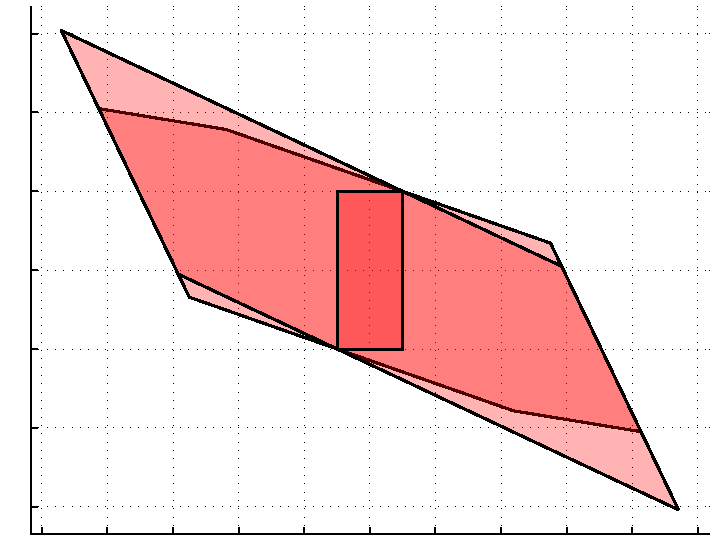
\includegraphics[scale=0.6]{twoDimensional}}
\caption{The extremal MRPI sets $\mathcal Z^\infty\vert_{({\bf{0}},\theta_{min})}$ and $\mathcal Z^\infty
\vert_{({\bf{0}},\theta_{\max})}$ containing the unit box.}
\label{fig:two:dim:example}
\end{figure}
\begin{figure}
\centerline{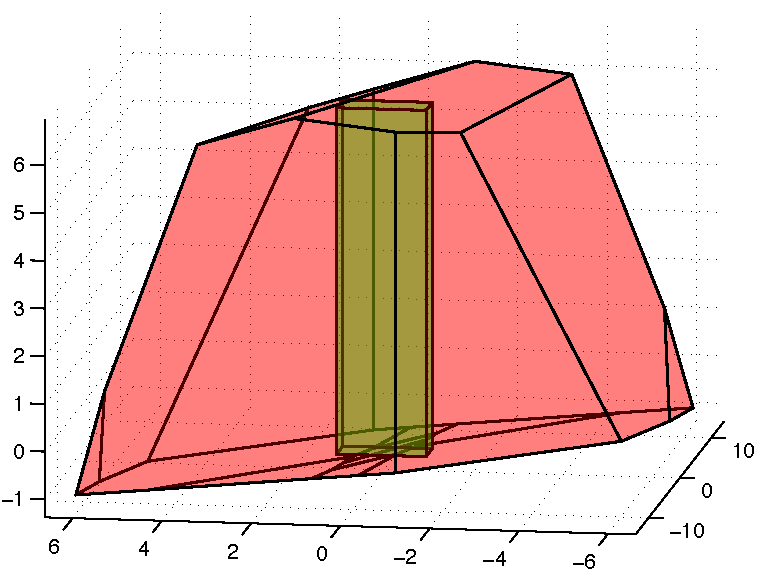
\includegraphics[scale=0.6]{threeDimensional}}
\caption{The parametrised MRPI set for $\alpha={\bf{0}}$. Containing the unit box in the 
interior between $\theta_{\min}$ and $\theta_{\max}$.}
\label{fig:three:dim:example}
\end{figure}
%
%
%
\section{Conclusions}\label{sec:conclusions}
%
In this paper we discussed extensions to existing computational methods to determine MRPI sets
for linear systems subject to additive disturbance in two cases. The case of state dependent case
which can be applied to determine approximations to MRPI sets for linearised nonlinear systems as was shown
for the example of a levitating ball system. We also introduced the computation of MRPI sets using 
scaling parameters which allows various system analyses using uniform scaling for the disturbance sets
and non-uniform scaling for the input constraints. The effectiveness of state dependent disturbance
sets was demonstrated by comparing the two MRPI methods.
\bibliographystyle{IEEEtran}
\bibliography{IEEEabrv,MyLib}
%
\end{document}